\begin{mdframed}[style=warning]
	\begin{ejercicio}
		\textbf{Conceptos.}
		\begin{enumerate}
			\item Una superficie tiene un vector de área $\vec{A} = \qty(2\vi + 3\vj)m^2$. Cuál es el flujo de un campo eléctrico uniforme a travez del área si el campo es (a) $\vec{E} = 4\vi N/C$ y (b) $\vec{E} = 4\vk N/C$?
			\item Considere 3 cilindros centrados en el mismo eje. El cilindro central (cilindro A) tiene carga uniforme igual a $q_A = +3q_o$. Qué cargas uniformes deberían de tener los otros dos cilindros (B y C) para que el campo eléctrico neto sea cero en las 3 regiones posibles (entre A y B, entre B y C y fuera de C)?
		\end{enumerate}
	\end{ejercicio}
\end{mdframed}






\begin{mdframed}[style=warning]
	\begin{ejercicio}
		Utilizando el modelo de Thomson, considere un átomo que contiene dos electrones, cada uno con carga $-e$, inmersos en una esfera de carga $+2e$ y radio $R$. En el equilibrio, cada electrón a una distancia $d$ del centro del átomo. Calcule la distancia $d$ en términos de las demás propiedades del átomo.
	\end{ejercicio}
\end{mdframed}











\begin{mdframed}[style=warning]
	\begin{ejercicio}
		Una distribución de carga no uniforme, pero con simetría esférica, tiene la densidad de carga $\rho (r)$ dada como sigue:
		$$
			\left.\begin{array}{cc}
				\rho (r) = \rho _o (1 - r/R) & \text{para} \, r\leq R \\
				\rho (r) = 0 & \text{para} \, r\geq R
			\end{array}\right.
		$$
		donde $\rho _o = 3Q/\pi R^3$ es una constante positiva. \textit{a)} Demuestre que la carga total contenida en la distribución de carga es $Q$. \textit{b)} Demuestre que el campo eléctrico en la región $r\geq R$ es idéntico al que produce una carga puntual $Q$ en $r = 0$. \textit{c)} Obtenga una expresión para el campo eléctrico en la región $r \leq R$. \textit{d)} Elabore la gráfica de la magnitud del campo eléctrico $E$ como función de $r$. \textit{e)} Encuentre el valor de $r$ para el que el campo eléctrico es máximo y calcule el valor deese campo máximo.
	\end{ejercicio}
\end{mdframed}















\begin{mdframed}[style=warning]
	\begin{ejercicio}
		Una esfera sólida no conductora con densidad carga volumétrica uniforme $\rho$. Sea $\vec{r}$ el vector desde el centro de la esfera a cualquier punto $P$ dentro de la esfera. (a) Demuestre que el el campo eléctrico en $P$ está dado por $\vec{E} = \flatfrac{\rho \vec{r}}{3\varepsilon _o}$. (b) Una cavidad esférica es sacada de la esfera, como se muestra en la figura. Demuestre que el campo eléctrico en la cavidad es uniforme e igual a $\vec{E} = \flatfrac{\rho \vec{a}}{3\varepsilon _o}$, donde $\vec{a}$ es el vector de posición desde el centro de la esfera hasta el centro de la cavidad.
		\begin{figure}[H]
			\centering
			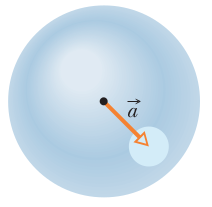
\includegraphics[scale=0.5]{./img/sphere.png}
			\caption{Esfera con cavidad.}
			\label{sphere}
		\end{figure}
	\end{ejercicio}
\end{mdframed}










































%%%